\clearpage
\section{碎石表面的高度}
在 Forge 里打开 \path{assets/scenes/Relief-Study.redflag}，选中“砂石”，在“模型绘制”里展开“部件 1 的材质”。“高度贴图效果”的四个选项共用同一张灰度图。图上白色代表最高处，黑色代表最低处。示例把两者的距离设为 0.055 米，让人从斜上方也能看清差别。这个数是展台的设置，调小之后，石面会渐渐变平。

\begin{center}
\panelimage{.485\linewidth}{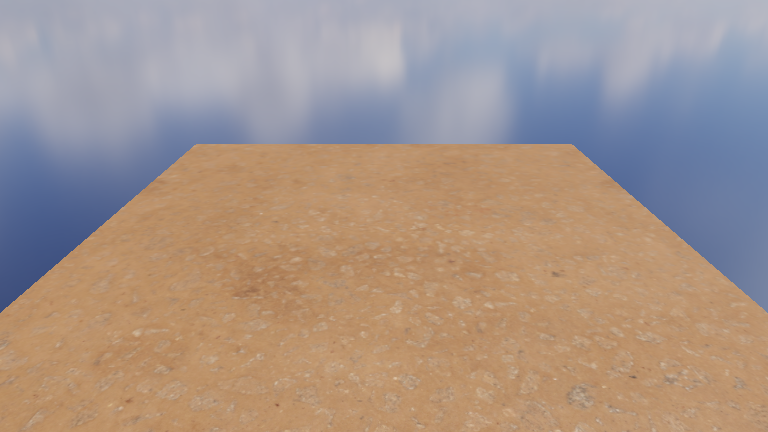
\includegraphics[width=\linewidth]{../../../output/validation/material-height/off.png}}{关闭高度。观察砂石的亮斑和地块边缘。}\hfill
\panelimage{.485\linewidth}{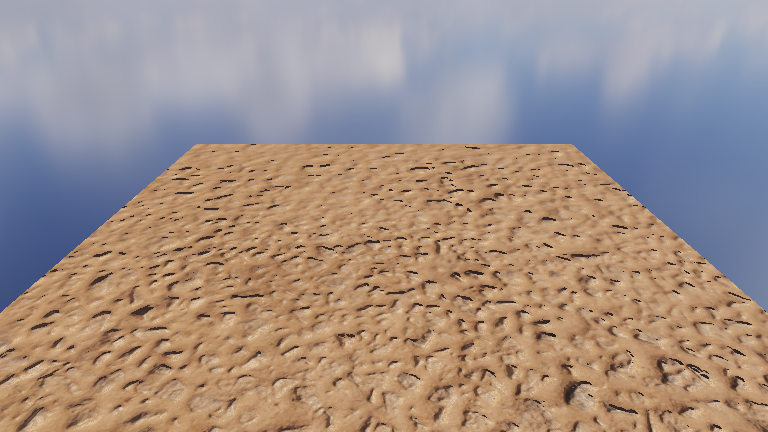
\includegraphics[width=\linewidth]{../../../output/validation/material-height/bump.png}}{凹凸。石子的两侧有了朝光和背光之分。}\\[5pt]
\panelimage{.485\linewidth}{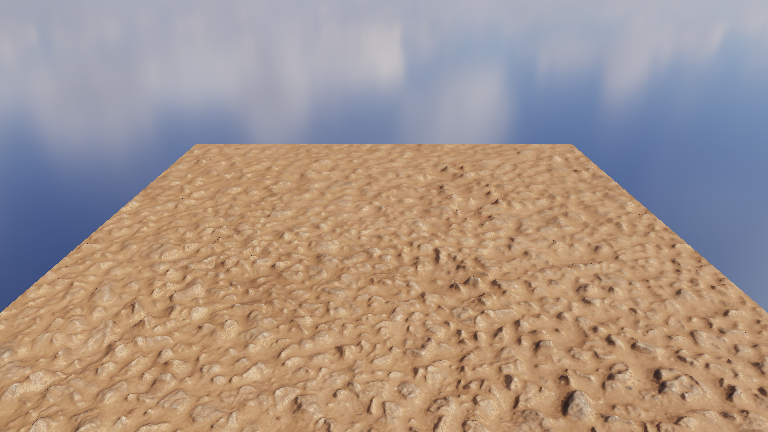
\includegraphics[width=\linewidth]{../../../output/validation/material-height/parallax.png}}{视差遮蔽。斜看时，凹处的纹理偏向一侧。}\hfill
\panelimage{.485\linewidth}{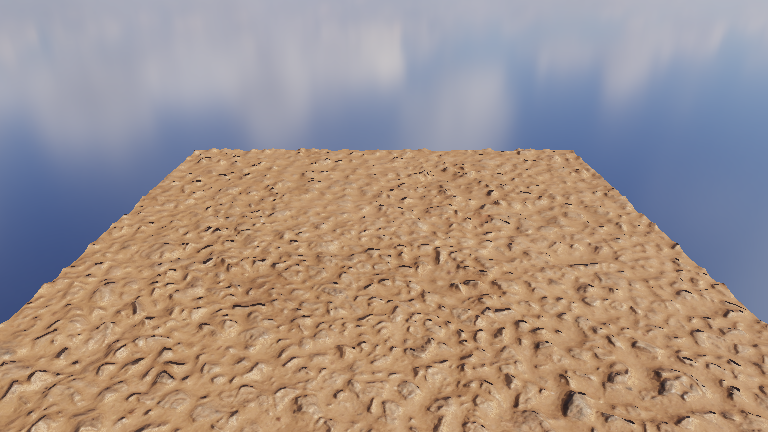
\includegraphics[width=\linewidth]{../../../output/validation/material-height/displacement.png}}{顶点置换。远处贴着天空的边缘也有了起伏。}
\end{center}

把相邻两处相差的高度除以水平距离，就得到这段表面的坡度。凹凸贴图（bump mapping）分别在贴图左右和上下取样，用这两个坡度算出表面朝向，也就是光照需要的法线。光从左上方照来时，一颗石子的两侧因而能有不同亮度。三角形仍在原处，选中地块的范围也和第一张图相同。

换成视差遮蔽（parallax occlusion mapping）后，要先算眼睛能看到石面的哪一点。设视线与表面法线夹角为 $\theta$。在一块平地上向下走 $d$ 米，沿视线水平方向就会错开 $d\tan\theta$ 米。从正上方看，$\theta=0$，底色不用挪动。斜看时，着色器把这段距离换算成贴图坐标，沿路比较视线的深度与高度图读到的深度。第一次越过石面，就在前后两次取样之间求交点，再用交点去读底色和粗糙度。进入更深的缝隙，需要向前多找几次。

\readings{\refitem{https://learnopengl.com/Advanced-Lighting/Parallax-Mapping}{LearnOpenGL，Steep Parallax Mapping 及 Parallax Occlusion Mapping}；
\refitem{https://polyhaven.com/a/gravel_road}{Amal Kumar，Gravel Road，CC0}。四张图均为本项目 Vulkan 实拍。}

\clearpage
\subsection{顶点、轮廓与绘制时间}
顶点置换直接改变石面的位置。设 $g$ 是高度图读到的数（黑为 0，白为 1），$H$ 是材质中填写的黑白高度差，$\boldsymbol n$ 是指向表面外侧的单位法线。顶点原来在 $\boldsymbol p$，现在移到
\[
 \boldsymbol p'=\boldsymbol p-\boldsymbol n\,H(1-g).
\]
例如 $H=0.055$ 米、$g=0.4$ 时，这个顶点向内移动 3.3 厘米。显卡仍然在三个顶点之间画一个平面。示例的两米地块每边分成 64 段，边缘能跟着高低起伏；一张只有四个角的平面读不到中间石子的形状。

\noindent\path{Redflag/src/Platform/Vulkan/Shaders/Mesh.vert}，顶点阶段的 \code{main}，下列变量名与源码相同。
\begin{lstlisting}
// 白色的顶点留在原地，黑色的顶点向内移动整个高度差。
float depth = 1.0 - textureLod(heightMap, a_TexCoord, 0.0).r;
position.xyz -= a_Normal * (heightRange() * depth);
\end{lstlisting}
片元阶段在 \path{Shaders/HeightSurface.glsl} 的 \code{bumpNormal} 求坡度，在 \code{reliefUV} 找视线与石面的交点。项目为正对镜头的表面选 8 层，斜看时最多 24 层。加密分层能分辨更窄的沟槽，也会增加读贴图的次数。高度为零时，绘制恢复到原材质。

{\smalltable\noindent\begin{tabularx}{\linewidth}{@{}Xrrr@{}}\toprule
同一块砂石 & CPU 录制（微秒）& GPU 绘制（微秒） & GPU P10--P90\\\midrule
关闭高度 & 40.15 & 17.712 & 17.54--17.92\\
凹凸 & 40.05 & 18.720 & 18.63--19.96\\
视差遮蔽 & 40.00 & 45.376 & 44.22--45.76\\
顶点置换 & 39.70 & 19.040 & 18.85--19.23\\\bottomrule
\end{tabularx}}

固定镜头和日光，用 RTX 5070 Ti Laptop GPU 在 $768\times432$ 下绘制，每种模式都是一次调用、8,192 个三角形。CPU 一栏是 Debug 构建录制这次场景绘制的 32 帧中位数。GPU 一栏是 RenderDoc 1.47 回放写入底色、法线和深度这一事件的 12 次中位数。视差的耗时随表面占据的像素和观察角变化，此处只能比较同一块地上的四种选择。

逐像素检查中，凹凸只改了法线；视差还改变了 183,935 个像素的底色；顶点置换改变了 188,020 个像素的深度和 6,018 个像素的拾取编号。三种模式现用于 Vulkan 的不透明材质。碰撞与静态间接光采样继续使用导入模型的几何。实际阈值、原图、截帧摘要及未测的纹理压缩方案见 \path{output/validation/material-height/README.md}。

\readings{\refitem{https://developer.nvidia.com/gpugems/gpugems2/part-i-geometric-complexity/chapter-8-pixel-displacement-mapping-distance-functions}{William Donnelly，GPU Gems 2，第 8.1 节，比较表面朝向与几何置换}。}
